\chapter{Implementation}

\section{Camera driver}

The camera driver was implemented based on Linux Video for Linux second version (V4L2) framework. It is a great framework that supports varies kinds of different camera sensor models with the same user space interface, across vast number of different embedded Linux platforms, enables cross platform adaptability with accessibility to low level controls.

For adaptive operation, the driver implemented supports different resolution modes from the camera and changing frame interval in great precision. A special control instruction that can change any of the control registers inside the camera sensor was also developed for debugging and controlling purpose.

A GPIO connected to a LED on the camera module was also controllable through the driver, to give indications about camera activity, used for debugging purpose and triggering external power analyser.

\section{Application}

% {\color{red}Application structure, multithreading}
% Bayer pattern handling.
% Multi-threading:
% 	i. Camera thread for camera control, buffer swapping, synchronisation and management etc.
% 	ii. OpenGL preview thread shows the camera output in real time, can be suspended for power saving.
% 	iii. OpenCV worker thread running algorithms.
% 	iv. OpenCV viewing thread.
% 	Display results and handle GUI user input, slow, can be suspended for power saving.

\subsection{Bayer pattern handling}

A typical colourful computer image consists of 3 primary colour channels {\color{red}CITE}, which are red, green and blue. However, because of physical and manufacture constrains, most of camera sensors including the camera used in this project have only one intensity sensor per pixel of a specific colour, arranged in a special pattern called Bayer pattern {\color{red}CITE}, therefore image processing algorithm need to be applied to convert or approximate the raw data to produce full colour images. Some of the camera sensors have a built-in image processor that applies the algorithm automatically, but the camera used in this project doesn't have that functionality, therefore the algorithm need to be implemented by the application.

{\color{red}Some diagrams show how it is done.}

\subsection{Application structure}

An application was developed to receive video stream from the camera or read continuous frame images from the dataset, then apply OpenCV processing, real-time input and output video preview as well as camera control. To take the benefits of the heterogeneous architecture more efficiently and overcome issues with buffer updates, the application was implemented using a multi-threading approach with inter-thread synchronisation mechanisms.

The main thread is responsible for initialisation, camera control, capture buffer synchronisation and management. It allocates several buffers for the camera driver, assign filled buffers to other processing threads and recycle processed buffers back to camera driver.

Afterwards, an OpenGL video preview thread was used to show the frames captured from camera to a monitor, independent from algorithm processing. This thread can be independently stalled so that it would not consume any processing power when analysing performances and power consumptions of algorithms.

The OpenCV algorithms runs on both CPU and GPU, and OpenCV has a constrain that to view the processed images, the application needs to call a user interface update function that is time consuming but not power intensive, therefore 2 threads was used in a pipeline style in order to speed up the processing. The buffers received from main thread will first go through the processing thread, then pass to the second thread for display on the monitor. The display thread can also be stalled for power saving.

%The OpenCV algorithms runs on both CPU and GPU, therefore to take the full advantages of heterogeneous architecture and run the algorithms as fast as possible, the OpenCV processing runs in a pipelined style through 3 threads. Every buffer received will go through first CPU processing thread, then transferred to GPU processing thread, finally .
%and OpenCV has a constrain that to view the processed image results, the application, so that two OpenCV processing threads was created so that.

Finally, an input handing thread for debugging and controlling through command line interface. Most of time this thread is block waiting for user input, therefore won't consume considerable CPU time.

\section{Object detection algorithms}

\subsection{Colour based}

An simple implementation \cite{MOTBOC.git} of colour filtering object detection algorithm was investigated, as shown in \fref{Figure:MOTBOC}.

{\color{red}UPDATE!}
\begin{figure}[H]
  \centering
  \includegraphics[width=0.6\columnwidth]{"MOTBOC failure"}
  \caption{Simple multi object tracking based on colour \cite{MOTBOC.git} in ideal situation}
  \label{Figure:MOTBOC_F}
\end{figure}

However, this implementation is very limited, it can only detects objects with single colour, cannot distinguish the objects from similar background colour, relies heavily on manually adjusted colour threshold values, and is very sensitive to the variations of colour spaces from different cameras, therefore not very adaptable. A complex environment may also results into lots of undesired detections, as shown in \fref{Figure:MOTBOC_F}.

\begin{figure}[H]
  \centering
  \includegraphics[width=0.6\columnwidth]{"MOTBOC failure"}
  \caption{Simple multi object tracking based on colour \cite{MOTBOC.git} at a complex environment}
  \label{Figure:MOTBOC_F}
\end{figure}

{\color{red}Descriptions about the failure}

\subsection{Shape based}

OpenCV's implementation of Hough Circle Transform for circle detection was investigated, as shown by \fref{Figure:circles}.

%\fref{Figure:circles} shows the image processed by circle detection, based on OpenCV's implementation of Hough Circle Transform \cite{opencv:hough_circle}.

\begin{figure}[H]
  \centering
  \subfigure [] {
    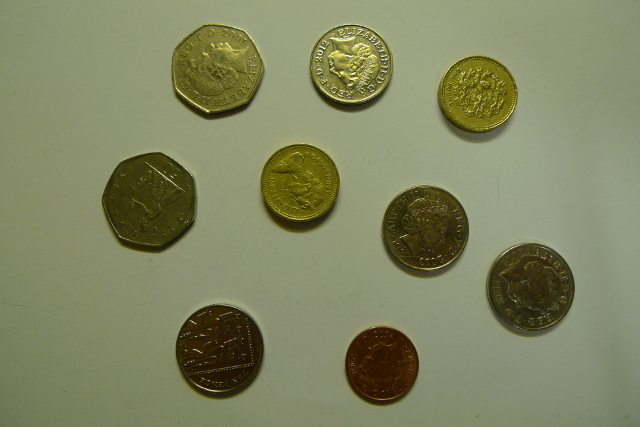
\includegraphics[width=0.45\columnwidth]{simple_original}
    \label{Figure:edges:original}
  }
  \subfigure [] {
    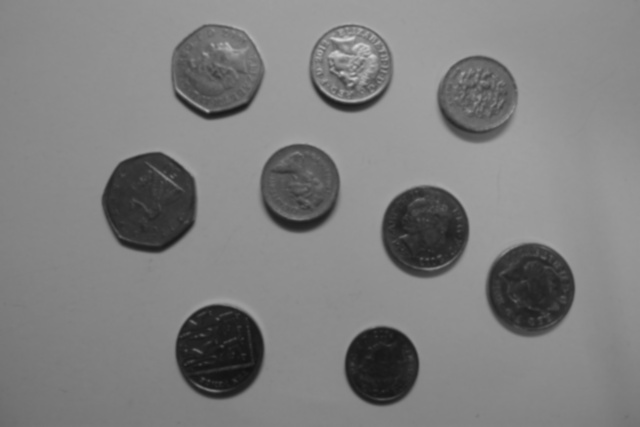
\includegraphics[width=0.45\columnwidth]{simple_blur}
    \label{Figure:edges:blur}
  }
  \subfigure [] {
    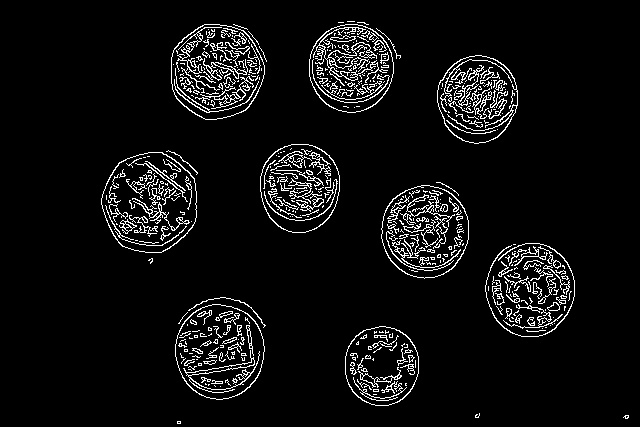
\includegraphics[width=0.45\columnwidth]{simple_edges}
    \label{Figure:edges:edges}
  }
  \subfigure [] {
    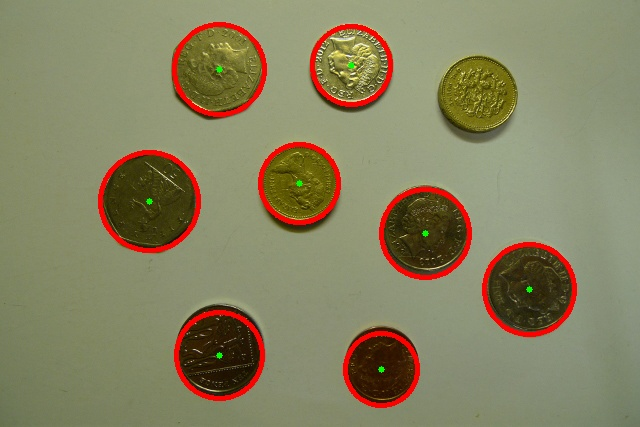
\includegraphics[width=0.45\columnwidth]{simple_circles}
    \label{Figure:edges:circles}
  }
  \caption{Circle detection. \subref{Figure:edges:original} The original image, \subref{Figure:edges:blur} image converted to gray scale and blurred, \subref{Figure:edges:edges} edges detected, \subref{Figure:edges:circles} circles detected}
  \label{Figure:circles}
\end{figure}

The frame captured from camera (\fref{Figure:edges:original}), was first converted to grey scale then blurred, as shown in \fref{Figure:edges:blur}. Blur or smoothing is often necessarily to reduce false object edges that might be detected. Afterwards the object edges in the image was extracted as in \fref{Figure:edges:edges}. Finally \fref{Figure:edges:circles} shows the circles detected by the algorithm.

However, this algorithm is still very limited and inaccurate, as shown by \fref{Figure:circles}, the coin at the top right corner had not been detected, because it appeared to be an eclipse instead of a prefect circle to the algorithm because of camera perspective. Furthermore, in order to detect multiple geometric shapes, different algorithms would be required for each of the different shapes.

\subsection{Cascade Classifier}

% as shown in \fref{Figure:cc_face}

The OpenCV's cascade classifier implementation \cite{opencv:cc} of face and eye detection was investigated as shown in \fref{Figure:cc_face}.

\begin{figure}[H]
  \centering
  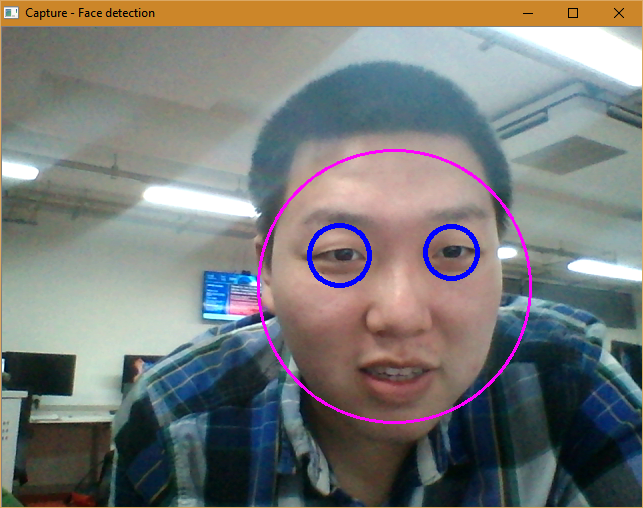
\includegraphics[width=0.6\columnwidth]{cc_imp_face}
  \caption{Face and eye detection cascade classifiers, detected face was circled by pink, whereas detected eyes were circled by blue}
  \label{Figure:cc_face}
\end{figure}

Noticeable {\color{red}DATA?} frame rate drop and latency was experienced (about only {\color{red}xx} fps) when experiments with the cascade classifier implementation on the testing platform, suggests it might not be a suitable algorithm for real-time object tracking application on embedded platforms.

\subsection{Motion based}

This article \cite{bgs:article} reviewed the algorithms available in the BGSLibrary, ranked 5 algorithms as the best methods for accuracy, 4 of 5 algorithms listed in \tref{Table:bgs} were investigated in this project.

{\color{red}GPU implementation?}

\iffalse
\begin{table}[H]
  \centering
  \begin{tabular}{cc}
  \toprule
  \textbf{Method ID} & \textbf{Method name}\\
  \midrule
  MultiLayerBGS & Multi-Layer BGS \\
  MixtureOfGaussianV1BGS & Gaussian Mixture Model \\
  LBAdaptiveSOM & Adaptive SOM \\
  DPWrenGABGS & Gaussian Average \\
  \bottomrule
  \end{tabular}
  \caption{Background substraction algorithms investigated (adapted from \cite{bgslibrary})}
  \label{Table:bgs}
\end{table}
\fi

The missing algorithm is Pixel-Based Adaptive Segmenter (PBAS), because the algorithm is based on patented ViBE algorithm, therefore removed from the BGSLibrary to avoid patent issue. However, the ViBE algorithm was existed in early versions of OpenCV as a non-free add-on module implemented with CUDA runs on GPU, therefore the ViBE algorithm was also investigated.

\fref{Figure:bgs_frame} shows the foreground masks obtained from those 4 algorithms through 2 sample frame sequences available with the BGSLibrary \cite{bgslibrary}.

{\color{red}ViBE}

\begin{figure}[H]
  \centering
  \includegraphics[width=0.24\columnwidth]{bgs_frame/MultiLayerBGS/input}
  \includegraphics[width=0.24\columnwidth]{bgs_frame/MultiLayerBGS/mask}
  %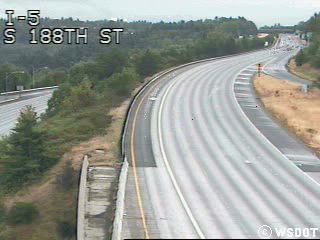
\includegraphics[width=0.32\columnwidth]{bgs_frame/MultiLayerBGS/bkgmodel}
  \includegraphics[width=0.24\columnwidth]{bgs_video/MultiLayerBGS/input}
  \includegraphics[width=0.24\columnwidth]{bgs_video/MultiLayerBGS/mask}

  \includegraphics[width=0.24\columnwidth]{bgs_frame/MixtureOfGaussianV1BGS/input}
  \includegraphics[width=0.24\columnwidth]{bgs_frame/MixtureOfGaussianV1BGS/mask}
  \includegraphics[width=0.24\columnwidth]{bgs_video/MixtureOfGaussianV1BGS/input}
  \includegraphics[width=0.24\columnwidth]{bgs_video/MixtureOfGaussianV1BGS/mask}
  %
\includegraphics[width=0.32\columnwidth]{na}

  \includegraphics[width=0.24\columnwidth]{bgs_frame/LBAdaptiveSOM/input}
  \includegraphics[width=0.24\columnwidth]{bgs_frame/LBAdaptiveSOM/mask}
  \includegraphics[width=0.24\columnwidth]{bgs_video/LBAdaptiveSOM/input}
  \includegraphics[width=0.24\columnwidth]{bgs_video/LBAdaptiveSOM/mask}
  %
\includegraphics[width=0.32\columnwidth]{na}

  \includegraphics[width=0.24\columnwidth]{bgs_frame/DPWrenGABGS/input}
  \includegraphics[width=0.24\columnwidth]{bgs_frame/DPWrenGABGS/mask}
  \includegraphics[width=0.24\columnwidth]{bgs_video/DPWrenGABGS/input}
  \includegraphics[width=0.24\columnwidth]{bgs_video/DPWrenGABGS/mask}
  %
\includegraphics[width=0.32\columnwidth]{na}
  \caption{Results obtained from background subtraction algorithms. From left to right column: input sample 1, foreground mask obtained, input sample 2, foreground mask obtained. From top to bottom row: MultiLayerBGS, MixtureOfGaussianV1BGS, LBAdaptiveSOM and DPWrenGABGS.}
  \label{Figure:bgs_frame}
\end{figure}

{\color{red}Background truth, how to tell best masks?}

It can be seen from \fref{Figure:bgs_frame} that MultiLayerBGS gave the best foreground masks, but it was also the slowest algorithm on the testing platform.

\section{Object tracking algorithms}

%Connected component analysis or blob detection (\sref{blob}) and movement tracking (\sref{bg:tracking}) algorithms were not implemented yet.

%A suitable camera module need to be ordered and interfaced afterwards, then implement automatic feedback control of frame rate, cropping and down sampling.

\subsection{Connected component analysis}

\subsection{Continuously Adaptive Meanshift}

\subsection{Optical flow}

\section{Adaptive power saving operation}

\section{Video stream dataset}
